\makeatletter
\def\maxwidth#1{\ifdim\Gin@nat@width>#1 #1\else\Gin@nat@width\fi}
\makeatother

\chapter{Background}

In this chapter, I presented the background knowledge to build a Delta Robot. The advantages and disadvantages of a robot with a parallel mechanisms are described. A review of different parallel mechanisms and their industrial application is presented. 
In section 2.3, I described about the kinematics solution of the Delta robot, which is the most important issue to design Delta robot.
The chapter closes with two section introduction to the Arduino and A4988.

\section{Robotics}

The word robot was introduced in 1921 by the Czech playwright Karel Capek in his satirical play R. U. R. (Rossum’s Universal Robots),where he depicted robots as machines which resembled people but worked tirelessly The structure of a robot is usually mostly mechanical and can be called a kinematic chain. The system structures of a robot varies depending on the task it will perform. A typically industrial robot is the serial robot which is built up by an open kinematic chain. This chain can be described as links connected to each other with revolute joints driven by actuators. This type of structure is often seen in the car industry.
The history of industrial automation is characterized by periods of rapid change in popular methods. Either as a cause or, perhaps, an effect, such periods of change in automation techniques seem closely tied to world economics. Along with computer aided design (CAD) systems, and computer aided manufacturing (CAM) systems the industrial robot became identifiable as a unique device, in the 1960’s (2). The robots are growing in complexity and their use in industry is becoming more widespread. This leads to new structures with different advantages and disadvantages\cite{intro_robotic_thesis}.

Parallel structures as the Delta robot possess a number of advantages when compared with serial manipulators. They offer generally a much higher rigidity and smaller mobile mass than their serial counterparts. Thus, they can move a much heavier payload relative to the components of body mass compared to a serial manipulator. The system structure of a Delta robot also makes it more stiff perpendicular to the traveling plate (e.g. resistive against vibration perpendicular to the traveling plate). The major drawback of the parallel robots is their limited range of motion compared to a serial robot, but with a system structure as the Delta robot, this limitation has partially been resolved.

\begin{table}[H]
\centering
\caption{Characteristics of serial and parallel robots\cite{compare_serial_parallel_robots_thesis}}
\label{tab:Characteristics_of_serial_and_parallel_robots}
\begin{tabular}{|l|l|l|}
\specialrule{.2em}{.1em}{.1em}
\textbf{Feature}                & \textbf{Serial robot} & \textbf{Parallel robot} \\ \specialrule{.2em}{.1em}{.1em}
Workspace                       & Large      			& Small and complex       \\ \hline
Solving forward kinematics      & Easy  				& Very \\ \hline
Solving inverse kinematics      & Difficult             & Easy                     \\ \hline
Position error                  & Accumulates           & Averages                 \\ \hline
Force error                     & Averages              & Accumulates              \\ \hline
Maximum force                   & \begin{tabular}[c]{@{}l@{}}Limited by minimum\\ actuator force\end{tabular} & \begin{tabular}[c]{@{}l@{}}Summation of all\\ actuator forces\end{tabular}           \\ \hline
Stiffness                       & Low                   & High                     \\ \hline
Dynamics characteristics        & \begin{tabular}[c]{@{}l@{}}Poor, especially with \\ increasing the size\end{tabular} & Very high             \\ \hline
\begin{tabular}[c]{@{}l@{}}Modelling andsolving \\ dynamics\end{tabular} & Relatively simple     & Very complex       \\ \hline
Inertia                         & Large                 & Small                    \\ \hline
Areas ofapplication             & \begin{tabular}[c]{@{}l@{}}A great number in \\ different areas, \\ especially in industry\end{tabular} & \begin{tabular}[c]{@{}l@{}}Currently limited, \\ especially in industry\end{tabular} \\ \hline
Payload/weight ratio            & Low                   & High                     \\ \hline
Speed andacceleration           & Low                   & High               		\\ \hline
Accuracy                        & Low                   & High                   	\\ \hline
Uniformity ofcomponents         & Low                   & High                      \\ \hline
Calibration                     & Relatively simple     & Complicated               \\ \hline
Workspace/robot size ratio      & High                  & Low               		\\ \hline
\end{tabular}
\end{table}

Inconclusion, with the purpose of serving for the Automated Mobile App Testing System, I need a robotic arm have high speed, stable and accurate operation in small space. From the pros cons were analyzed above, I decided to choose Parallel robot(Delta robot) for my testing system.

\section{Delta Robot}

It is in the early 80's when Reymond Clavel (professor at EPFL - École Polytechnique Fédérale de Lausanne) comes up with the brilliant idea of using parallelograms to build a parallel robot with three translational and one rotational degree of freedom. Contrary to opinions published elsewhere, his inspiration was truly original and does not come from a parallel mechanism patented by Willard L. Pollard in 1942, which at that time was not known to Professor Clavel. The latter calls his creation the Delta robot, without suspecting that at the turn of the century, it will establish itself as one of the most successful parallel robot designs, with several hundred active robots worldwide. In 1999, Dr. Clavel is presented with the Golden Robot Award, sponsored by ABB Flexible Automation, for his innovative work on the Delta parallel robot\cite{intro_deltarobot_thesis}. 
\subsection{The Design}
\begin{figure}[H]
	\centering
	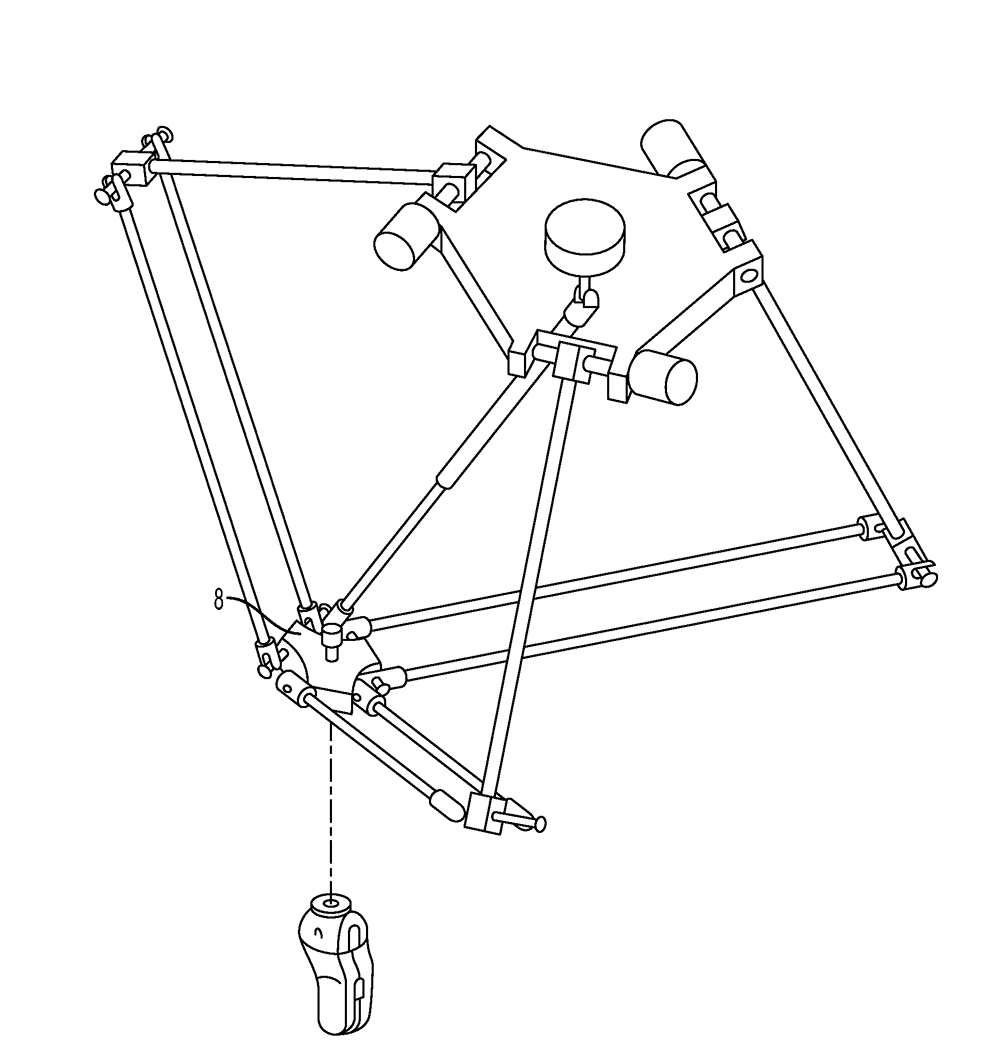
\includegraphics[width=\maxwidth{15cm}, keepaspectratio]{Chapters/Fig/deltarobot_first_design.png}
	\caption{Original technical drawing from U.S Patent n.4,976,582\cite{US_patent_deltarobot_thesis}}
	\label{fig:deltarobot_first_design}
\end{figure}

The basic idea behind the Delta parallel robot design is the use of parallelograms. A parallelogram allows an output link to remain at a fixed orientation with respect to an input link. The use of three such parallelograms restrain completely the orientation of the mobile platform which remains only with three purely translational degrees of freedom. The input links of the three parallelograms are mounted on rotating levers via revolute joints. The revolute joints of the rotating levers are actuated in two different ways: with rotational (DC or AC servo) motors or with linear actuators. Finally, a fourth leg is used to transmit rotary motion from the base to an end-effector mounted on the mobile platform\cite{intro_deltarobot_thesis}.

The use of base-mounted actuators and low-mass links allows the mobile platform to achieve accelerations of up to 50 G in experimental environments and 12 G in industrial applications. This makes the Delta robot a perfect candidate for pick and place operations of light objects (from 10 gr to 1 kg). Ideally, its workspace is the intersection of three right circular tori. The Delta robots available on the market operate typically in a cylindrical workspace which is 1 m in diameter and 0.2 m high.

\subsection{Application}

Industries that take advantage of the Delta robot’s high speed are the packaging, medical and pharmaceutical industries. Other possible applications include assembly tasks or operation in a clean room for electronic components. More recently, Delta robot is the low-cost solution to build 3D printer for about a few hundred dollars from RepRap project\cite{reprap_thesis}. The Delta robot’s structure can also be used to build a Automated System Testing for mobile phone.

\section{Delta robot kinematics}

To build delta robot we need to solve two problems. Firstly, given the desired position of the end effector (for example, to catch a pancake in the point with coordinates $x$,$y$,$z$), it is necessary to determine the corresponding angles of each of three arms (joint angles) in order to set the motors (and, thereby, the end effector) in proper position for grasping. This process is known as inverse kinematics. 

And, secondly, if the joint angles are known (for example, by reading the values of the motor encoders), it is necessary to determine the position of the end effector (i.e. to make some corrections regarding its current position). This is known as a forward kinematics problem. 

To be more formal, let's look at the kinematic scheme of the delta robot. The platforms are two equilateral triangles: the fixed triangle with the motors is green, and the movable triangle with the end effector is pink. The joint angles are $\theta_{1}$, $\theta_{2}$ and $\theta_{3}$, and the point is the end effector’s position with coordinates ($x_{0}$, $y_{0}$, $z_{0}$).
To solve inverse kinematics problems we have to create a function with the coordinates ($x_{0}$, $y_{0}$, $z_{0}$) of as parameters, which returns ($\theta_{1}$, $\theta_{2}$, $\theta_{3}$). A forward kinematics function uses ($\theta_{1}$, $\theta_{2}$, $\theta_{3}$) to return ($x_{0}$, $y_{0}$, $z_{0}$).
\begin{figure}[H]
	\centering
	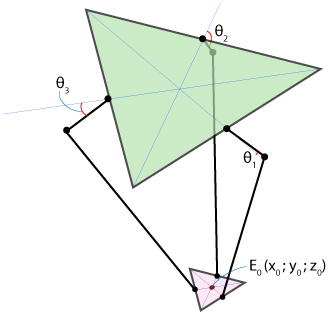
\includegraphics[width=\maxwidth{12cm}, keepaspectratio]{Chapters/Fig/kinematic_scheme.png}
	\caption{Kinematic scheme of the delta robot}
	\label{fig:kinematic_scheme}
\end{figure}
\subsection{Inverse kinematics}
\begin{figure}[H]
	\centering
	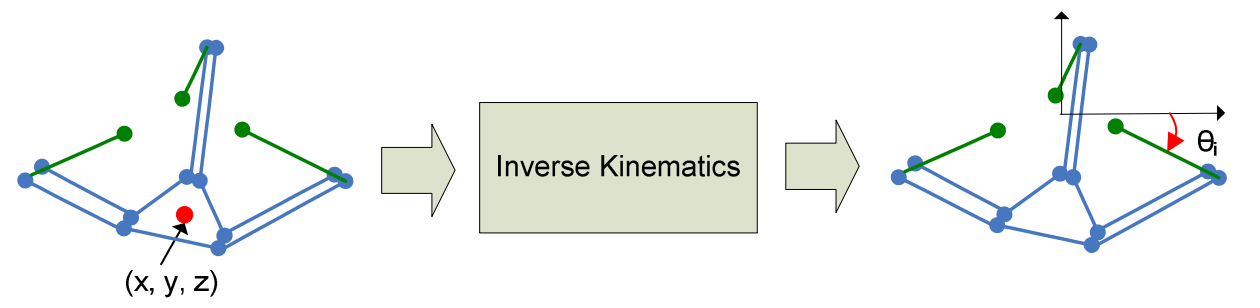
\includegraphics[width=\maxwidth{15cm}, keepaspectratio]{Chapters/Fig/inverse_kinematics.png}
	\caption{inverse kinematics transforms the robots position (x,y,z) into the three upper arm angle positions $\theta_{1}$, $\theta_{2}$, $\theta_{3}$}
	\label{fig:inverse_kinematics}
\end{figure}
\subsubsection{Some key parameters}

First, let's determine some key parameters of our robot's geometry. Let's designate the side of the fixed triangle as $f$, the side of the end effector triangle as $e$, the length of the upper joint as $r_{f}$,  and the length of the parallelogram joint as $r_{e}$. These are physical parameters that are determined by the robot. The reference frame will be chosen with the origin at the fixed triangle's centre of symmetry, as shown below, so that the z-coordinate of the end effector will always be negative.
\begin{figure}[H]
	\centering
	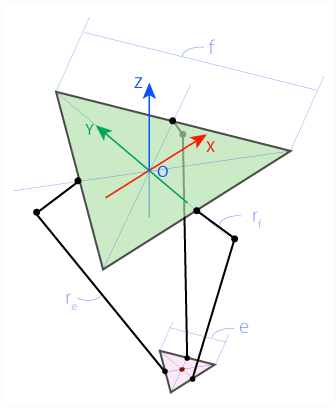
\includegraphics[width=\maxwidth{12cm}, keepaspectratio]{Chapters/Fig/key_parameters.png}
	\caption{Some key parameters of our robot's geometry}
	\label{fig:key_parameters}
\end{figure}
Because of the robot's design, joint $\overline{F_{1}J_{1}}$ can only rotate in the YZ plane (see fig. below), forming a circle centered in point $F_{1}$ with radius $r_{f}$. Unlike $F_{1}$, $J_{1}$ and $E_{1}$ are so-called universal joints, which means that $\overline{E_{1}J_{1}}$ can rotate freely relatively to $E_{1}$, forming a sphere centered in point $E_{1}$ with radius $r_{e}$.
\begin{figure}[H]
	\centering
	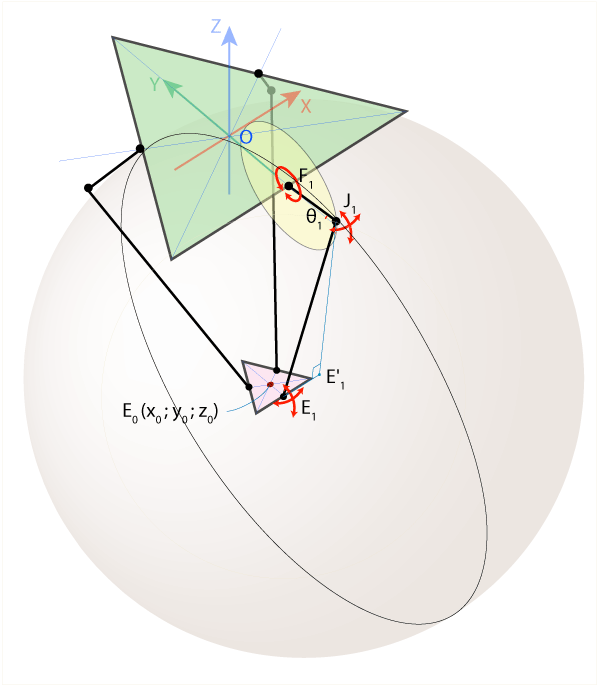
\includegraphics[width=\maxwidth{12cm}, keepaspectratio]{Chapters/Fig/find_point_J1.png}
	\caption{Find point $J_{1}$}
	\label{fig:find_point_J1}
\end{figure}
The intersection of this sphere and the YZ plane is a circle centered in point $E^{'}_{1}$ with radius $\overline{E^{'}_{1}J_{1}}$, where $E^{'}_{1}$ is the projection of the point $E_{1}$ on the YZ plane. The point can be found now as the intersection of two circles of known radius centered in $E^{'}_{1}$ and $F_{1}$ respectively (we should choose only one intersection point with a smaller Y-coordinate). And if we know $J_{1}$, we can calculate the angle of $\theta_{1}$.
Such algebraic simplicity follows from our good choice regarding the frame of reference, which causes joint $\overline{F_{1}J_{1}}$ to move in the YZ plane only. As such, we can completely omit the X coordinate.
\subsubsection{Equations}
\begin{figure}[H]
	\centering
	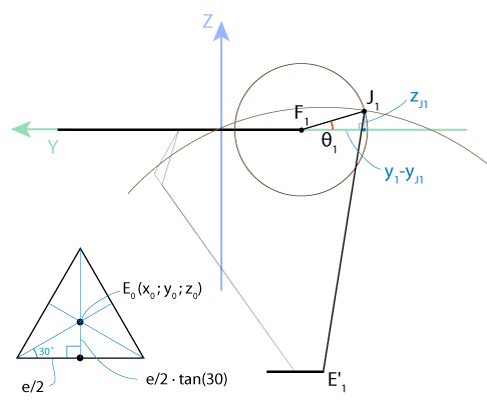
\includegraphics[width=\maxwidth{13cm}, keepaspectratio]{Chapters/Fig/find_theta1.png}
	\caption{Find $\theta_{1}$}
	\label{fig:find_theta1}
\end{figure}
\begin{flalign*}
& E_{0} = (x_{0}, y_{0}, z_{0}) &\\
& \overline{EE_{1}} = \frac{e}{2}\tan 30 = \frac{e}{2\sqrt{3}} &\\
& E_{1} = \left (x_{0}, y_{0} - \frac{e}{2\sqrt{3}}, z_{0} \right ) \Rightarrow E^{'}_{1} = \left (0, y_{0} - \frac{e}{2 \sqrt{3}}, z_{0} \right ) & \\
& \overline{EE_{1}} = x_{0} \Rightarrow \overline{E^{'}_{1}J_{1}} = \sqrt{\overline{E_{1}J_{1}^{2}} - \overline{E_{1}E^{'}_{1}}^{2}} = \sqrt{r^{2}_{e} - x^{2}_{0}} & \\
& F_{1} = \left (0, - \frac{f}{2\sqrt{3}}, 0 \right ) & \\
& \begin{cases}
 & (y_{J_{1}} - y_{F_{1}})^{2} + (z_{J_{1}} - z_{F_{1}})^{2} = r^{2}_{f}\\ 
 & (y_{J_{1}} - y_{E^{'}_{1}})^{2} + (z_{J_{1}} - z_{E^{'}_{1}})^{2} = r^{2}_{e} - x^{2}_{0}
\end{cases} \\
& \Rightarrow 
\begin{cases}
 & (y_{J_{1}} - \frac{f}{2\sqrt{3}})^{2} + z_{J_{1}}^{2} = r^{2}_{f} \\ 
 & (y_{J_{1}} - y_{0} + \frac{e}{2\sqrt{3}})^{2} + (z_{J_{1}} - z_{0})^{2} = r^{2}_{e} - x^{2}_{0}
\end{cases} \\
& \Rightarrow J_{1} = (0, y_{J_{1}}, z_{J_{1}}) & \\
& \theta_{1} = \tan^{-1}\left ( \frac{z_{J_{1}}}{y_{F_{1}} - y_{J_{1}}} \right ) & \\
\end{flalign*}

For the remaining angles $\theta_{2}$ and $\theta_{3}$, we should take advantage of the delta robot's symmetry. First, let's rotate the XY plane 120 degrees counterclockwise around the Z-axis, as it is shown below. 
We've got a new reference frame X'Y'Z', and with this frame we can find the angle $\theta_{2}$ using the same algorithm that we used to find $\theta_{1}$. The only change is that we need to determine new coordinates $x^{'}_{0}$ and $y^{'}_{0}$ for the point $E_{0}$, which can be easily done using the corresponding rotation matrix. To find the angle $\theta_{3}$ we have to rotate the frame of reference clockwise, starting from the initial position.
\begin{figure}[H]
	\centering
	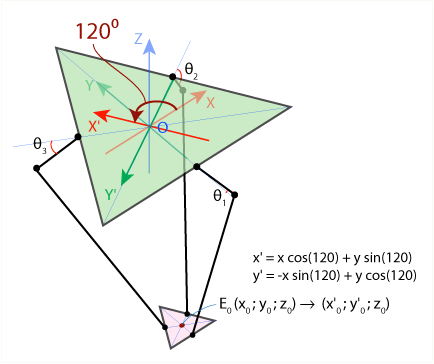
\includegraphics[width=\maxwidth{13cm}, keepaspectratio]{Chapters/Fig/find_theta2_and_theta3.png}
	\caption{Find $\theta_{2}$ and $\theta_{3}$}
	\label{fig:find_theta2_and_theta3}
\end{figure}

\subsection{Forward kinematics}
\begin{figure}[H]
	\centering
	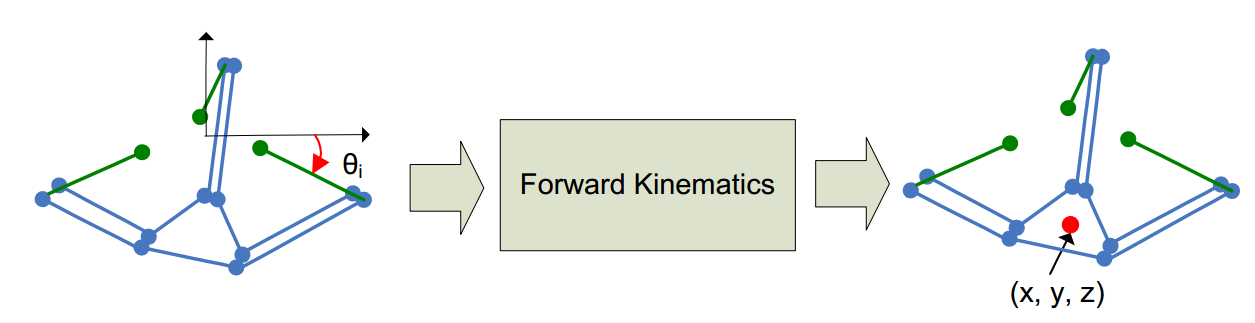
\includegraphics[width=\maxwidth{15cm}, keepaspectratio]{Chapters/Fig/forward_kinematics.png}
	\caption{Forward kinematics transforms the three arm angle positions $\theta_{1}$, $\theta_{2}$, $\theta_{3}$ into the x,y and z}
	\label{fig:forward_kinematics}
\end{figure}
\subsubsection{Some key parameters}

Now that the three joint angles ($\theta_{1}$, $\theta_{2}$, $\theta_{3}$) are known, and we need to find the coordinates ($x_{0}$, $y_{0}$, $z_{0}$) of the end effector point $E_{0}$.
Since we know the angles, we can easily find the coordinates of points $J_{1}$, $J_{2}$ and $J_{3}$ (see fig. below).
Joints $\overline{J_{1}E_{1}}$, $\overline{J_{2}E_{2}}$ and $\overline{J_{3}E_{3}}$ can freely rotate around points $J_{1}$, $J_{2}$ and $J_{3}$ respectively, forming three spheres with radius $r_{e}$.
\begin{figure}[H]
	\centering
	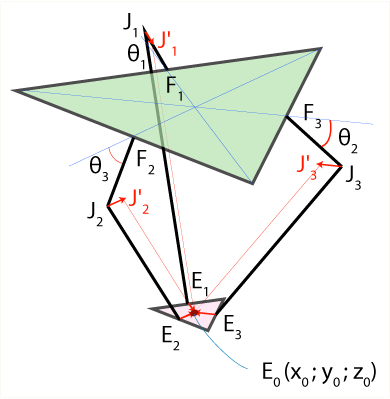
\includegraphics[width=\maxwidth{13cm}, keepaspectratio]{Chapters/Fig/forward_kinematics_key_parameters.png}
	\caption{Key parameters of forward kinematics}
	\label{fig:forward_kinematics_key_parameters}
\end{figure}
Now let's do the following: move the centers of the spheres from points , and to points $J_{1}$, $J_{2}$ and $J_{3}$ using transition vectors $\overline{E_{1}E_{0}}$, $\overline{E_{2}E_{0}}$ and $\overline{E_{3}E_{0}}$ respectively. After this transition all three spheres will
intersect in one point: $E_{0}$, as shown in the figure below:
\begin{figure}[H]
	\centering
	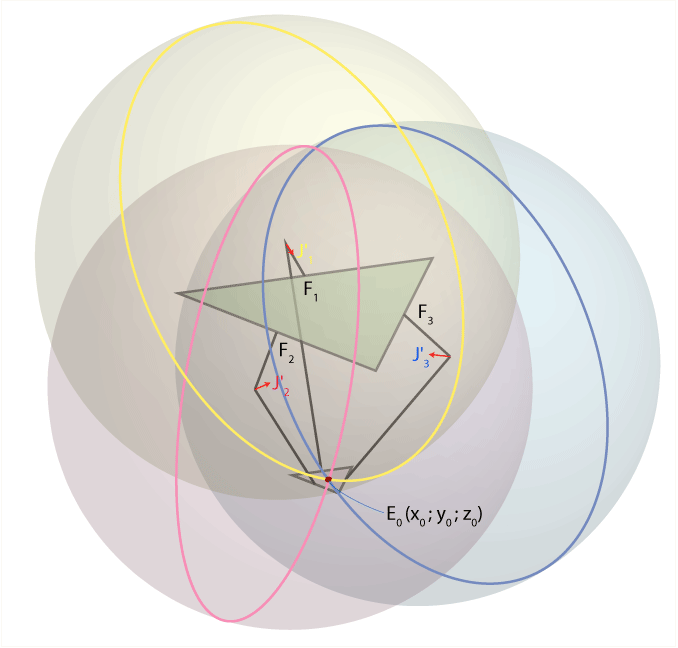
\includegraphics[width=\maxwidth{13cm}, keepaspectratio]{Chapters/Fig/intersection_of_three_spheres.png}
	\caption{Intersection of three spheres}
	\label{fig:intersection_of_three_spheres}
\end{figure}
\subsubsection{Equations}

So, to find the coordinates ($x_{0}$, $y_{0}$, $z_{0}$) of the point $E_{0}$, we need to solve a set of three equations like
$$(x - x_{j})^{2} + (y - y_{j})^{2} + (z - z_{j})^{2} = r^{2}_{e}$$
where the coordinates of sphere centers ($x_{j}$, $y_{j}$, $z_{j}$) and the radius $r_{e}$ are known. First, let's find the coordinates of points $J^{'}_{1}$, $J^{'}_{2}$, $J^{'}_{3}$:
\begin{figure}[H]
	\centering
	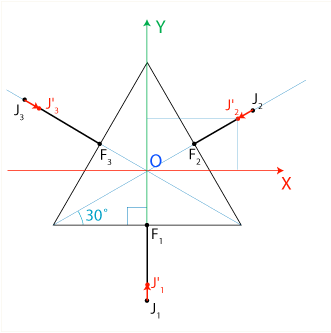
\includegraphics[width=\maxwidth{12cm}, keepaspectratio]{Chapters/Fig/find_J1_J2_J3_coordinates.png}
	\caption{Find $J^{'}_{1}$, $J^{'}_{2}$, $J^{'}_{3}$ coordinates}
	\label{fig:find_J1_J2_J3_coordinates}
\end{figure}
\begin{flalign*}
& OF_{1} = OF_{2} = OF_{3} = \frac{f}{2\tan30} = \frac{f}{2\sqrt{3}} & \\
& J_{1}J^{'}_{1} = J_{2}J^{'}_{2} = J_{3}J^{'}_{3} = \frac{e}{2\tan30} = \frac{e}{2\sqrt{3}} & \\
& F_{1}J_{1} = r_{f}\cos(\theta_{1}) & \\
& F_{2}J_{2} = r_{f}\cos(\theta_{2}) & \\
& F_{3}J_{3} = r_{f}\cos(\theta_{3}) & \\
& J^{'}_{1}(0; \frac{-(f-e)}{2\sqrt{3}} - r_{f}\cos{\theta_{1}}; -r_{f}\sin(\theta_{1})) & \\
& J^{'}_{2}(\left [\frac{(f-e)}{2\sqrt{3}} + r_{f}\cos{\theta_{2}}  \right]\cos(30); \left [\frac{(f-e)}{2\sqrt{3}} + r_{f}\cos{\theta_{2}}  \right]\sin(30); -r_{f}\sin(\theta_{2})) & \\
& J^{'}_{3}(\left [\frac{(f-e)}{2\sqrt{3}} + r_{f}\cos{\theta_{3}}  \right]\cos(30); \left [\frac{(f-e)}{2\sqrt{3}} + r_{f}\cos{\theta_{3}}  \right]\sin(30); -r_{f}\sin(\theta_{3})) & \\
\end{flalign*}

In the following equations I'll designate the coordinates of points $J_{1}$, $J_{2}$, $J_{3}$ as ($x_{1}$, $y_{1}$, $z_{1}$), ($x_{2}$, $y_{2}$, $z_{2}$) and ($x_{3}$, $y_{3}$, $z_{3}$). Please note that $x_{0} = 0$. Here are the equations of the three spheres:

\begin{flalign*}
\begin{cases}
 x^{2} + (y - y_{1})^{2} + (z - z_{1})^2 = r^{2}_{e} \\ 
 (x - x_{2})^{2} + (y - y_{2})^{2} + (z - z_{2})^2 = r^{2}_{e}\\ 
 (x - x_{3})^{2} + (y - y_{3})^{2} + (z - z_{3})^2 = r^{2}_{e}\\ 
\end{cases} 
\end{flalign*}

$\Rightarrow$ 
\begin{numcases}{ }
x^{2} + y^{2} + z^{2} - 2y_{1}y - 2z_{1}z = r^2_{e} - y^{2}_{1} - z^{2}_{1} \label{fk_1}\\
x^{2} + y^{2} + z^{2} - 2x_{2}x - 2y_{2}y - 2z_{2}z = r^2_{e} - x^{2}_{2} - y^{2}_{2} - z^{2}_{2} \label{fk_2}\\ 
x^{2} + y^{2} + z^{2} - 2x_{3}x - 2y_{3}y - 2z_{3}z = r^2_{e} - x^{2}_{3} - y^{2}_{3} - z^{2}_{3} \label{fk_3}
\end{numcases}
\begin{flalign*}
w_{i} = x^{2}_{i} + y^{2}_{i} + z^{2}_{i}
\end{flalign*} 
\begin{numcases}{ }
x_{2}x + (y_{1} - y_{2})y + (z_{1} - z_{2})z = \frac{w_{1} - w_{2}}{2} \label{fk_4}\\ 
x_{3}x + (y_{1} - y_{3})y + (z_{1} - z_{3})z = \frac{w_{1} - w_{3}}{2} \label{fk_5}\\ 
(x_{2} - x_{3})x + (y_{2} - y_{3})y + (z_{2} - z_{3})z = \frac{w_{1} - w_{3}}{2} \label{fk_6} 
\end{numcases} 

From (\ref{fk_4}) - (\ref{fk_5}):
\begin{gather}
x = a_{1} + b_{1} \label{fk_7}\\
y = a_{2}z + b_{2} \label{fk_8}
\end{gather}
\begin{flalign*}
& a_{1} = \frac{1}{d}[(z_{2} - z_{1})(y_{3} - y_{1}) - (z_{3} - z_{1})(y_{2} - y_{1})] & \\
& a_{2} = \frac{1}{d}[(z_{2} - z_{1})x_{3} - (z_{3} - z_{1})x_{2}] & \\
& d = (y_{2} - y_{1})x_{3} - (y_{3} - y_{1})x_{2} & \\
\end{flalign*}

Now we can substitute (\ref{fk_7}) and (\ref{fk_8}) in (\ref{fk_1}):
\begin{flalign*}
& (a^{2}_{1} + a^{2}_{2} + 1)z^{2} + 2[a_{1} + a_{2}(b_{2} - y_{1}) - z_{1}]z + [b^{2}_{1} + (b_{2} - y_{1})^{2} + z^{2}_{1} - r^{2}_{e}] = 0 & \\
\end{flalign*}
And finally, we need to solve this quadric equation and find $z_{0}$ (we should choose the smallest negative root), and then calculate $x_{0}$ and $y_{0}$ from eq. (\ref{fk_7}) and (\ref{fk_8}).

\section{Arduino Mega 2560} 
% \cite{arduinomega_thesis}
\subsection{Overview}

The Mega 2560 is a microcontroller board based on the ATmega2560. The main structure of the Arduino Mega 2560 includes the following sections:
\begin{itemize}
		\item \textbf{USB connection}: This is the communication port to upload code from the PC to the microcontroller. It is also a serial interface for data transfer between the microcontroller and the PC.
		\item \textbf{Power jack}: USB connection can provide power to the device, but the microcontroller board can not alway be plugged to the computer. At that time we need a power supply with voltages from 9 to 12V.
		\item \textbf{54 digital input/output pins}: are numbered from 0 to 53(of which 15 can be used as PWM outputs).
		\item \textbf{16 analog inputs}
		\item \textbf{4 UARTs}: hardware serial ports.
\end{itemize}
\begin{figure}[H]
	\centering
	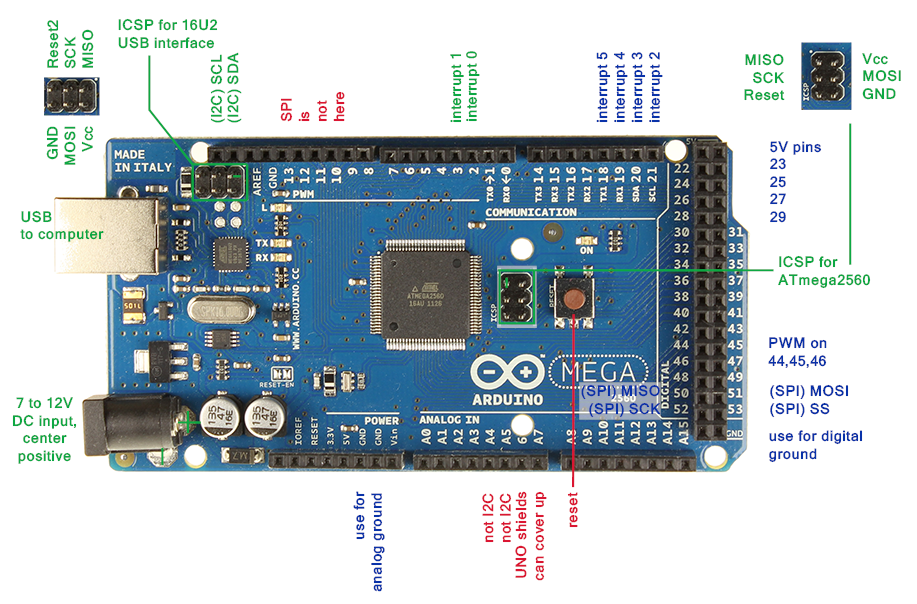
\includegraphics[width=\maxwidth{15cm}, keepaspectratio]{Chapters/Fig/arduinomega2560_pinouts.png}
	\caption{Arduino Mega 2560 R3 pinouts}
	\label{fig:arduinomega2560_pinouts}
\end{figure}
\subsection{Technical specs}
\begin{table}[H]
	\centering
	\caption{Arduino Mega 2560 technical specs\cite{arduinomega_thesis}}	
	\label{tab:arduinomega2560_technical_specs}
	\begin{tabularx}{0.65\textwidth}{ll}
		\toprule
		Microcontroller & ATmega2560 \\
		\midrule
		Operating Voltage & 5V \\
		\midrule 
		Input Voltage  & 7-12V \\
		(recommended)  & \\
		\midrule
		Input Voltage (limit) & 6-20V \\
		\midrule
		Digital I/O Pins & 54 \\
			& (of which 15 provide PWM output) \\
		\midrule
		Analog Input Pins & 16 \\
		\midrule
		DC Current per I/O Pin & 20 mA \\
		\midrule
		DC Current for 3.3V Pin & 50 mA \\
		\midrule
		Flash Memory & 256 KB of which 8 KB used by \\
			& bootloader \\
		\midrule
		SRAM & 8 KB\\
		\midrule
		EEPROM & 4 KB\\
		\midrule
		Clock Speed & 16 MHz\\
		\midrule
		Length & 101.52 mm\\
		\midrule
		Width & 53.3 mm\\
		\midrule
		Weight & 37 g \\
		\bottomrule
	\end{tabularx}
\end{table}
The Mega 2560 has 16 analog inputs, each of which provide 10 bits of resolution (i.e. 1024 different values). By default they measure from ground to 5 volts, though is it possible to change the upper end of their range using the AREF pin and analogReference() function.
The ATmega2560 has 256 KB of flash memory for storing code (of which 8 KB is used for the bootloader), 8 KB of SRAM and 4 KB of EEPROM (which can be read and written with the EEPROM library).
\newpage
\section{Stepper Motor and Driver A4988}
\subsection{Stepper Motor}

A stepper motor is an electromechanical device which converts electrical pulses into discrete mechanical movements. The shaft or spindle of a stepper motor rotates in discrete step increments when electrical command pulses are applied to it in the proper sequence. The motors rotation has several direct relationships to these applied input pulses. The sequence of the applied pulses is directly related to the direction of motor shafts rotation. The speed of the motor shafts rotation is directly related to the frequency of the input pulses and the length of rotation is directly related to the number of input pulses applied.
\subsubsection{Stepper Motor Advantages and Disadvantages}
\begin{itemize}
\item \textbf{Advantages}:
\begin{itemize}
\item The rotation angle of the motor is proportional to the input pulse.
\item The motor has full torque at standstill (if the windings are energized).
\item Precise positioning and repeatability of movement since good stepper motors have an accuracy of 3 – 5\% of a step and this error is non cumulative from one step to the next.
\item Excellent response to starting/stopping/reversing.
\item Very reliable since there are no contact brushes in the motor. Therefore the life of the motor is simply dependant on the life of the bearing.
\item The motors response to digital input pulses provides open-loop control, making the motor simpler and less costly to control.
\item It is possible to achieve very low speed synchronous rotation with a load that is directly coupled to the shaft.
\item A wide range of rotational speeds can be realized as the speed is proportional to the frequency of the input pulses.
\end{itemize}
\item \textbf{Disadvantages}:
\begin{itemize}
\item Resonances can occur if not properly controlled.
\item Not easy to operate at extremely high speeds.
\end{itemize}
\end{itemize}
\subsubsection{Stepper Motor System}
Operation of stepper motor is clearly shown in Figure:\ref{fig:theory_of_the_stepper_motor}
\begin{figure}[H]
    \centering
    \subfloat[One pulse equals one step]{{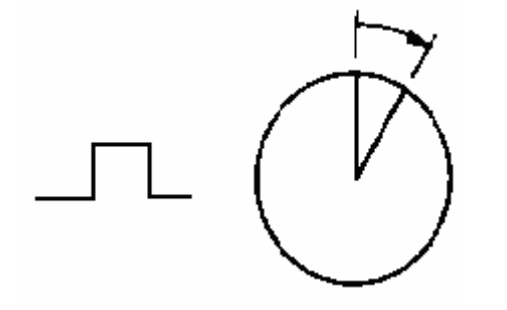
\includegraphics[width=7cm]{Chapters/Fig/one_step.png} }}%
    \qquad
    \subfloat[Pulse count equals step count]{{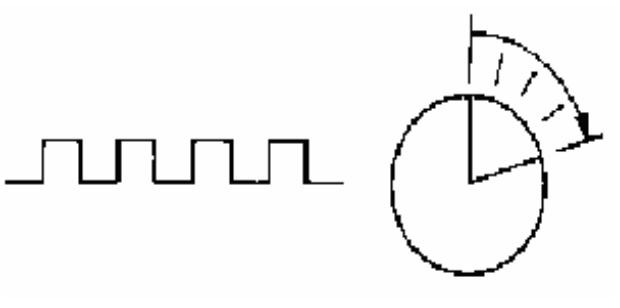
\includegraphics[width=7cm]{Chapters/Fig/multi_steps.png} }}%
    \caption{Theory of the stepper motor}%
    \label{fig:theory_of_the_stepper_motor}%
\end{figure}
Unlike DC or servo motors, step motors are synchronous devices. Any torque generated by the system is only the result of the load applied. These motors rely on input signals to step the rotor through discrete angles. A step motor system often contains three basic elements, as shown in the following figure:
\begin{figure}[H]
	\centering
	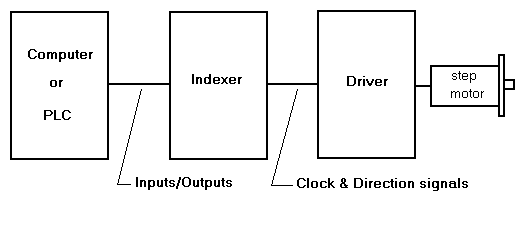
\includegraphics[width=\maxwidth{15cm}, keepaspectratio]{Chapters/Fig/stepper_motor_system.png}
	\caption{Stepper motor system overview}
	\label{fig:stepper_motor_system}
\end{figure}
The controller is a microprocessor(i.e. Arduino microcontroller,...) that directly processes the sophisticated high-level commands and provides step pulses and direction outputs to the driver. Usually, it is a programmable device and the programming process is accomplished with hardware switch settings. Most of applications require that the indexer manage other functions including acceleration, deceleration, drive resolution and distance as well. Microprocessor-based controller offer flexibility that they can operate in either stand-alone mode or interfaced to a host computer.

The main function of the driver is to convert the controller output signal into the power (voltage or current) necessary to drive the motor winding. One step pulse from the driver is required by one step advance of the motor shaft. In other word, the speed and torque performance of the step motor is based on the flow of current from the driver to the motor winding. Inductance, the most important parameter of the driver, refers to the time it takes for the current to energized the winding. In most industrial applications, driver circuits are designed to supply a greater amount of voltage than the voltage that drives the motors.

Generally speaking, the step motor itself consists of two parts, the stator and the rotor. The winding is the main part of the stator. Three-phase, four-phase and five-phase step motors have three, four and five windings, respectively. When in the working mode, the windings are energized in a specific order that is called the phase sequence. The rotor mainly composes a magnetic shaft. When the windings are energizing-deenergizing under the effect of the phase sequence signal, an electromagnetic field is generated around the rotor. Hence, the rotor starts rotating driven by the regular varied electromagnetic force.

The rotation angle of the motor is proportional to the input pulse, so we can accurately control in an open loop system. Open loop control means no feedback information about the position is needed. This type of control eliminates the need for expensive sensing and feedback devices such as optical encoders. Your position is known simply by keeping track of the input step pulses. This is the most significant advantages of a stepper motor.
\subsubsection{Stepper motor for Delta robot}
Using stepper motors is more difficult to get working, but they are superior in controllability, accuracy, and speed.

A NEMA 17 stepper motor is a stepper motor with a 1.7 x 1.7 inch (43.2 x 43.2 mm) faceplate\cite{reprap_nema17_thesis}.
\begin{itemize}
\item 1.5A to 1.8A current per phase
\item 1-4 volts
\item 3 to 8 mH inductance per phase
\item 44 N·cm (62oz·in, 4.5kg·cm) or more holding torque
\item 1.8 or 0.9 degrees per step (200/400 steps/rev respectively)
\end{itemize}
%NEMA 17 is the best suited for my Delta-robot 
\begin{figure}[H]
	\centering
	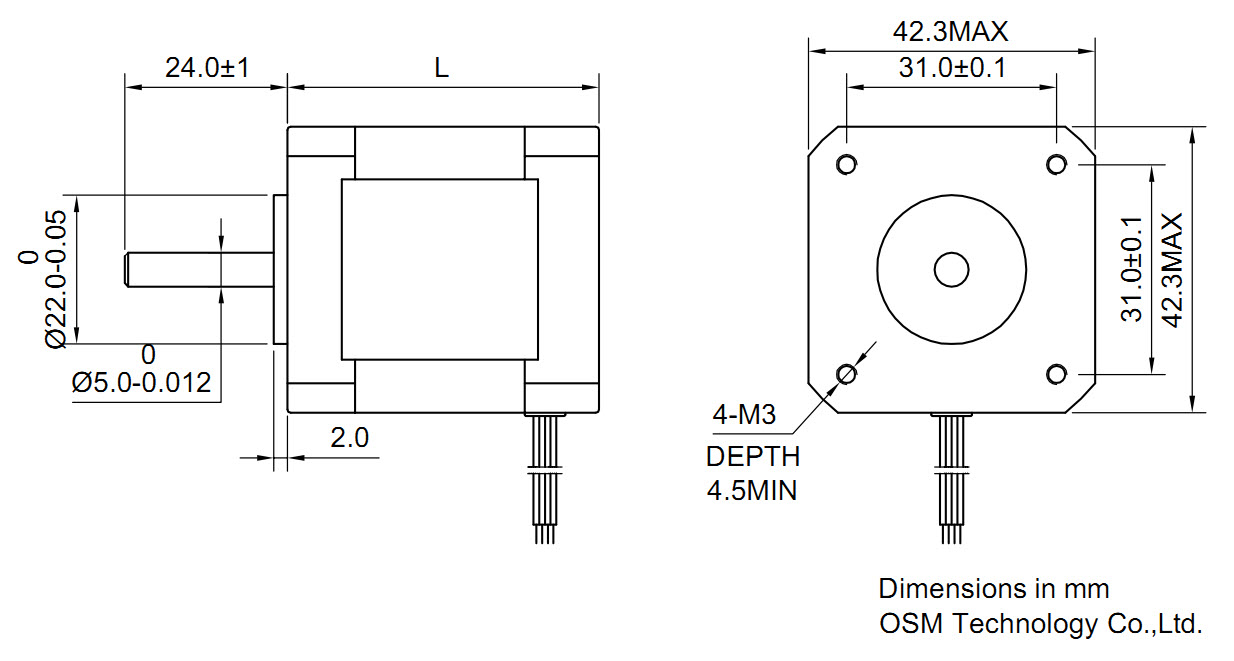
\includegraphics[width=\maxwidth{15cm}, keepaspectratio]{Chapters/Fig/nema_17_stepper_motor.jpg}
	\caption{NEMA-17 Stepper motor}
	\label{fig:nema_17_stepper_motor}
\end{figure}

\subsection{Driver A4988}

The Allegro's A4988 is a complete microstepping motor driver with built-in translator for easy operation. It is designed to operate bipolar stepper motors in full-, half-, quarter-, eighth-, and sixteenth-step modes, with an output drive capacity of up to 35 V and $\pm$2 A. The A4988 includes a fixed off-time current regulator which has the ability to operate in Slow or Mixed decay modes\cite{A4988_allegro_thesis}.

The translator is the key to the easy implementation of the A4988. Simply inputting one pulse on the STEP input drives the motor one microstep. There are no phase sequence tables, high frequency control lines,or complex interfaces to program. The A4988 interface is an ideal fit for applications where a complex microprocessor is unavailable or is overburdened. During stepping operation, the chopping control in the A4988 automatically selects the current decay mode, Slow or Mixed. In Mixed decay mode, the device is set initially to a fast decay for a proportion of the fixed off-time, then to a slow decay for the remainder of the off-time. Mixed decay current control results in reduced audible motor noise, increased step accuracy, and reduced power dissipation\cite{A4988_allegro_thesis}.

Internal synchronous rectification control circuitry is provided to improve power dissipation during PWM operation. Internal circuit protection includes: thermal shutdown with hysteresis, under voltage lockout (UVLO), and crossover-current protection. Special power-on sequencing is not required\cite{A4988_allegro_thesis}.

\subsubsection{Pololu - A4988 Stepper Motor Driver Carrier}
\begin{figure}[H]
	\centering
	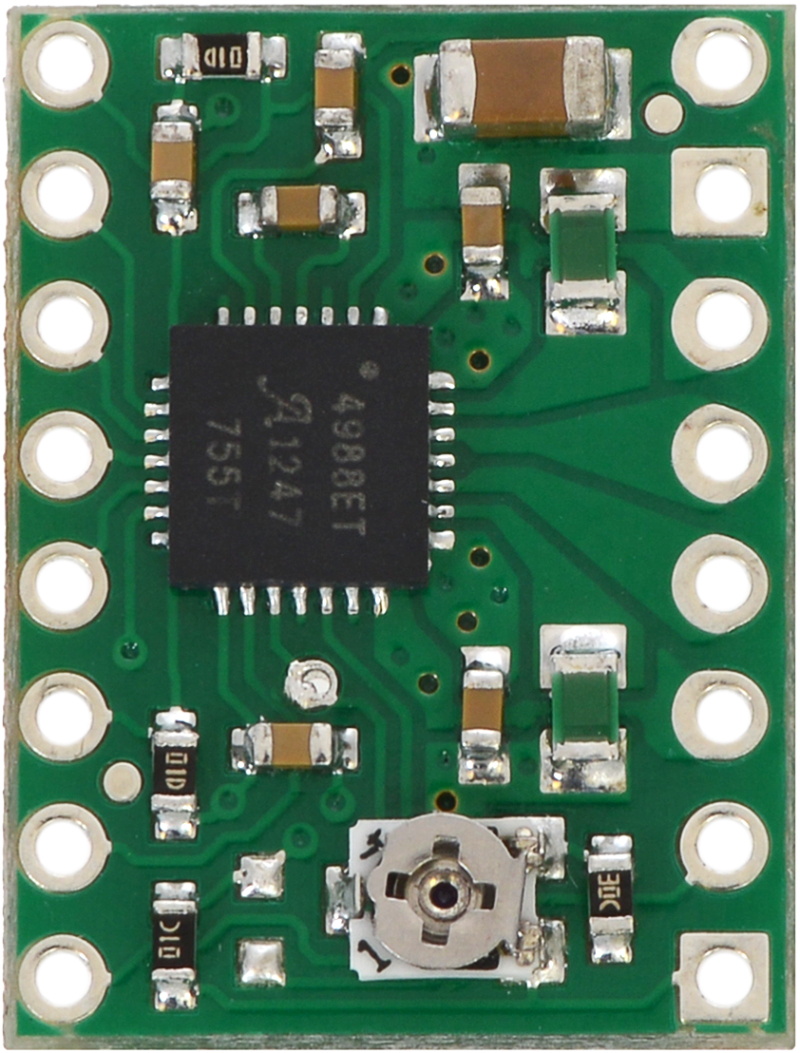
\includegraphics[width=\maxwidth{8cm}, keepaspectratio]{Chapters/Fig/pololu_A4988.jpg}
	\caption{Pololu - A4988 Stepper Motor Driver Carrier}
	\label{fig:pololu_A4988}
\end{figure}
This breakout board for Allegro's A4988 microstepping bipolar stepper motor driver features adjustable current limiting, over-current and over-temperature protection, and five different microstep resolutions (down to 1/16-step). It operates from 8 V to 35 V and can deliver up to approximately 1 A per phase without a heat sink or forced air flow (it is rated for 2 A per coil with sufficient additional cooling).

The driver's key features:
\begin{itemize}
\item Simple step and direction control interface.
\item Five different step resolutions: full-step, half-step, quarter-step, eighth-step, and sixteenth-step.
\item Adjustable current control lets you set the maximum current output with a potentiometer, which lets you use voltages above your stepper motor's rated voltage to achieve higher step rates.
\item Intelligent chopping control that automatically selects the correct current decay mode (fast decay or slow decay).
\item Over-temperature thermal shutdown, under-voltage lockout, and crossover-current protection.
\item Short-to-ground and shorted-load protection.
\end{itemize}

\subsubsection{Drive a Stepper Motor with an Arduino and a A4988}
\begin{figure}[H]
	\centering
	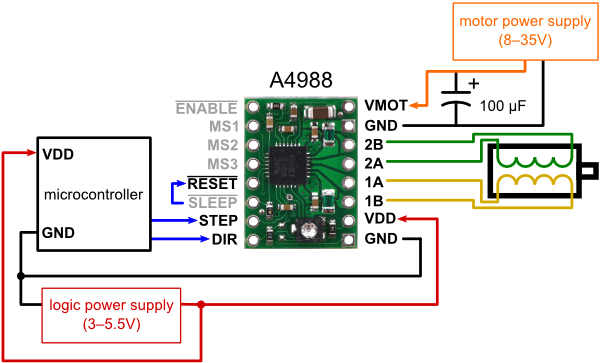
\includegraphics[width=\maxwidth{10cm}, keepaspectratio]{Chapters/Fig/minimal_wiring_diagram_pololu_A4988.png}
	\caption{Minimal wiring diagram for connecting a microcontroller to an A4988 stepper motor driver carrier (full-step mode)}
	\label{fig:minimal_wiring_diagram_pololu_A4988}
\end{figure}
The A4988 takes two digital inputs. One input sets the step direction, while the second is pulsed; each pulse commands the driver to advance one step (in the direction controlled by the direction pin). 

The specifications of a step command pulse are shown in Figure.\ref{fig:allegro_4988_logic_interface_timing_diagram} and Table.\ref{tab:allegro_4988_logic_interface_timing_diagram}.
\begin{figure}[H]
	\centering
	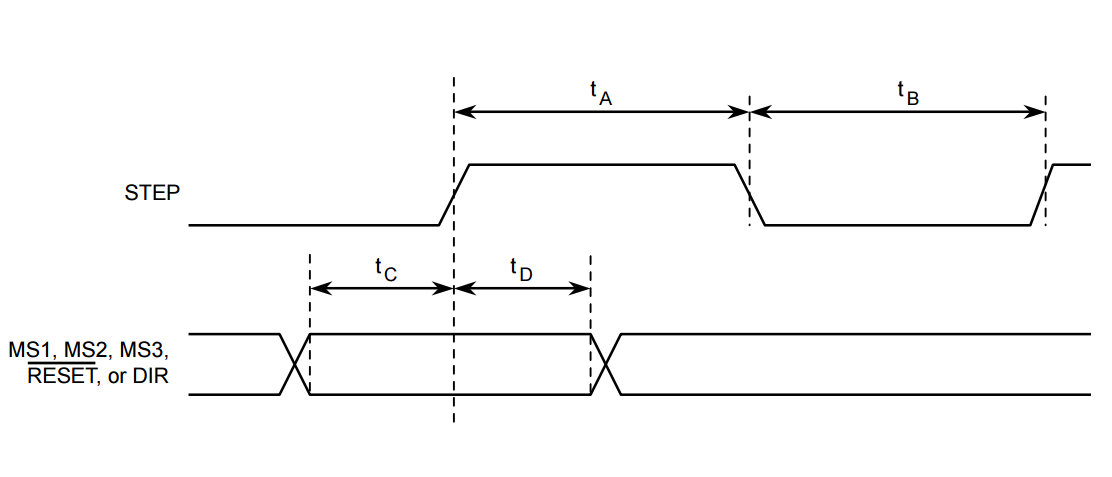
\includegraphics[width=\maxwidth{10cm}, keepaspectratio]{Chapters/Fig/allegro_4988_logic_interface_timing_diagram.png}
	\caption{Allegro 4988 logic interface timing diagram\cite{A4988_allegro_thesis}}
	\label{fig:allegro_4988_logic_interface_timing_diagram}
\end{figure}

\begin{table}[H]
	\centering
	\caption{Logic Interface Timing Diagram\cite{A4988_allegro_thesis}}
	\label{tab:allegro_4988_logic_interface_timing_diagram}
	\begin{tabular}{|l|l|l|l|l}
	\cline{1-4}
	Time Duration                    & Symbol 	   & Typ. & Unit 	 &  \\ \cline{1-4}
	STEP minimum, HIGH pulse width   & $t_{A}$     & 1    & $\mu$ s   &  \\ \cline{1-4}
	STEP minimum, LOW pulse width    & $t_{B}$     & 1    & $\mu$ s   &  \\ \cline{1-4}
	Setup time, input change to STEP & $t_{C}$     & 200  & $\mu$ s   &  \\ \cline{1-4}
	Hold time, input change to STEP  & $t_{D}$     & 200  & $\mu$ s   &  \\ \cline{1-4}
	\end{tabular}
\end{table}

To use A4988 driver we needs the following connections: 
\begin{itemize}
\item 4 connections to the stepper motor, marked 1A, 1B and 2A, 2B. Connect the first coil to 1A and 1B and the second coil to 2A and 2B.
\item Logic Power and GND, Connect this to the GND and +5V of the Arduino
\item Dir sets the direction the stepper will move.
\item Step will make the stepper step each time this pin goes form Low to High.
\item Enable. When this pin is pulled low the board is enabled and the motor energised. When set high the board is disabled and the motor is de-energised.
\item Sleep and Reset control the board, either sending it to sleep or resetting it. To use the board I tied these together which allows the board to run normally.
\item Motor Power and GND. This needs to be a high voltage/current supply to run the motor. I had a 12V, 2A wall Swart available(Do not connect this yet)
\item 3 pins (MS1, MS2 and MS3) are for selecting one of the five step resolutions are shown in the following Truth Table.\ref{tab:step_resolutions_truth_table}. These pins have internal pull-down resistors so if we leave them disconnected, the board will operate in full step mode.
\end{itemize}
\begin{table}[H]
\centering
\caption{Step resolutions truth table}
\label{tab:step_resolutions_truth_table}
\begin{tabular}{@{}llll@{}}
\toprule
\textbf{MS1} & \textbf{MS2} & \textbf{MS3} & \textbf{Resolution} \\ \midrule
LOW          & LOW          & LOW          & Full Step           \\
HIGH         & LOW          & LOW          & Haft Step           \\
LOW          & HIGH         & LOW          & Quarter Step        \\
HIGH         & HIGH         & LOW          & Eighth Step         \\
HIGH         & HIGH         & HIGH         & Sixteenth Step      \\ \bottomrule
\end{tabular}
\end{table}
\paragraph{Current Limiting}
To prevent damage to the driver chip, it uses circuitry to limit the maximum current that can be used. This is set via the adjustable resistor on the board, in co-operation with some of the other components, the sense resistors (S1 = 0.1Ohm and S2 = 0.1Ohm) and the resistor (R1 = 30kOhm).

According to the A4998 datasheet, and substituting those values, gives:
\begin{flalign*}
& V_{REF} max = (TrimpotMaxR/(TrimpotMaxR+R_{1})) * V_{DD} &\\
& = (10,000 / (10,000 + 30,000)) * 5 = 1.25V & \\
\end{flalign*}
The maximum value of current limiting is set by the selection of $R_{S}$ and the voltage at the VREF pin. The transconductance function
is approximated by the maximum value of current limiting, $I_{TripMAX}$ (A), which is set by: \\
$I_{TripMAX}$ (effectively max motor current) $= V_{REF}/(8 * R_{S})$
$ = 1.25/(8 * 0.1) = 1.5625A$ \\
To calculate amps from measured VREF: $A = V_{REF} / 0.8$ \\
To calculate VREF required for a target current: $V_{REF} = A * 0.8$ \\
\textbf{Example}: 
stepper motors are 0.4A. I can't get maximum current from this driver, however, if I drive them at 
70\% (0.4A x 70\% = 0.28A) I want to a $V_{REF}$ of 0.28A x 0.8 = 0.224V, plus driving them at 70\% will reduce the temperature of the stepper. \\
%I start with the trim pot turned anti-clockwise, and measure the voltage with my multimeter between the logic Gnd pin and the centre of the trimpot itself, slowly turning it up until I get just under 0.224V \\
\textbf{Warning}: Connecting or disconnecting a stepper motor while the driver is powered can destroy the driver. (More generally, rewiring anything while it is powered is asking for trouble.)